\documentclass[reprint,aps,prl,twocolumn,superscriptaddress,groupedaddress]{revtex4-2}

\usepackage[final]{graphicx}
\usepackage[hidelinks]{hyperref}
\usepackage{bm,physics,amsmath,amssymb,xcolor}
\usepackage[normalem]{ulem}

\usepackage{centernot}
\usepackage{braket}
\usepackage{tabularx}
\usepackage{booktabs}
\usepackage{pifont}
\usepackage{colortbl}
\usepackage{amsthm}
\usepackage{soul}
\usepackage{epsfig}

\setcounter{secnumdepth}{4}
\usepackage{titlesec}


% Custom commands
\newcommand{\eomo}{$E_1$-$M_1$}
\newcommand{\eoet}{$E_1$-$E_2$}
\newcommand{\etet}{$E_2$-$E_2$}
\newtheorem{theorem}{Theorem}
\newtheorem*{remark}{Theorem}
\definecolor{CL_Yellow}{HTML}{E69E5B}
\colorlet{LightYellow}{CL_Yellow!25}
\definecolor{CL_Pink}{HTML}{9E5BE6}
\colorlet{LightPink}{CL_Pink!25}
\definecolor{CL_Green}{HTML}{9EE65B}
\colorlet{LightBlue}{CL_Green!25}
\newcommand{\cg}[3]{C^{#1}_{#2;#3}}
\newcommand{\ii}{\mathrm{i}}

% Macros for commenting
\newcommand{\correction}[2]{\textcolor{red}{\sout{#1}} \textcolor{blue}{#2}}
\newcommand{\hide}[1]{}

% Command for getting figure size (in inches), font size and font name.
\usepackage{printlen}
\makeatletter
\edef\textFontName{\fontname\csname
  \f@encoding/\f@family/\f@series/\f@shape/\f@size\endcsname}
\edef\mathFontName{\fontname\textfont0}
\edef\mathLetterFontName{\fontname\textfont1}
\makeatother
\newcommand{\printsizes}{
    \uselengthunit{in}~\\
    textwidth: \printlength{\textwidth}\\
    linewidth: \printlength{\linewidth}\\
    text height: \printlength{\textheight}\\
    font name: \textFontName \\
    font size: \the\fontdimen6\font\relax
}


\begin{document}

\title{Bottom-up Analysis of Ro-Vibrational Helical Dichroism}

\author{Mateja Hrast}
\email[]{mateja.hrast@ist.ac.at}
\affiliation{Institute of Science and Technology Austria (ISTA), Am Campus 1, 3400 Klosterneuburg, Austria}
\author{Georgios M. Koutentakis}
\email{georgios.koutentakis@ist.ac.at}
\affiliation{Institute of Science and Technology Austria (ISTA), Am Campus 1, 3400 Klosterneuburg, Austria}
\author{Mikhail Maslov}
\email{mikhail.maslov@ist.ac.at}
\affiliation{Institute of Science and Technology Austria (ISTA), Am Campus 1, 3400 Klosterneuburg, Austria}
\author{Mikhail Lemeshko}
\email{mikhail.lemeshko@ist.ac.at}
\affiliation{Institute of Science and Technology Austria (ISTA), Am Campus 1, 3400 Klosterneuburg, Austria}

\date{\today}

%%%%%%%%%%%%%%%%%%%%%%%%%%%%%%%%%%%%%%%%%%%%%%%%%%%%%%%%%%%%%%%%%
\begin{abstract}
Helical dichroism (HD) is a proposed method for the resolution of molecular chirality, employing the orbital angular momentum (OAM) of light. Going beyond the conventional assumptions about~HD, this work proposes a rigid theoretical framework for the analysis of the HD, based on molecular symmetries and rotational eigenstates. We derive the rotational selection rules, which clearly establish that HD only emerges from the spin-orbit coupling of light, even for beams without far-field OAM. Our findings refine the conditions for observing HD, shedding light on the outcome of prior experiments and guiding future designs for chiral sensing using structured light.

\end{abstract}
%%%%%%%%%%%%%%%%%%%%%%%%%%%%%%%%%%%%%%%%%%%%%%%%%%%%%%%%%%%%%%%%%

\maketitle

%%%%%%%%%%%%%%%%%%%%%%%%%%%%%%%%%%%%%%%%%%%%%%%%%%%%
%              INTRODUCTION
%%%%%%%%%%%%%%%%%%%%%%%%%%%%%%%%%%%%%%%%%%%%%%%%%%%%

Many biologically and chemically important molecules exist as chiral pairs -- two non-superimposable mirror versions called enantiomers. The ability to separate the enantiomers is essential for the pharmaceutical and agrochemical industries \cite{MAIER2001}. This is perhaps best illustrated by the methamphetamine molecule, whose R-enantiomer is an effective nasal decongestant, while its S-enantiomer is a psychoactive drug that fuels addiction epidemics~\cite{barkholtz2023}. The high economic relevance has driven research on the asymmetric synthesis of chiral molecules,~e.g.,~via an enantioselective or bio-catalysis or by employing chiral auxiliaries \cite{Brown1989}. However, these advanced synthesis techniques require further refinement and the assessment of enantiomeric purity by enantio-selective processes. This next step, while essential, is still technically challenging. Existing chemical techniques each present their own challenges, ranging from high cost and time consumption to limited applicability and reliability \cite{qian2023}. Here, we address an alternative, chemical-physics perspective, aiming to assess enantiomeric purity through light–matter interactions. Owing to rapid advances in optical physics \cite{Koch2019}, this approach promises a cost-effective and highly controllable avenue for chiral discrimination.

For decades, the difference in absorption of left- and right-circularly polarised light, known as the circular dichroism (CD) \cite{deutsche1970,Holzwarth1974}, has been used in spectroscopy of chiral media \cite{Miles2021}. However, circular dichroism relies on a limited resource, namely the spin angular momentum of light. Meanwhile, pioneering optics work by Allen~\textit{et~al.}~\cite{Allen1992} has demonstrated that, in addition to spin, light also carries orbital angular momentum (OAM). In contrast to spin, the number of OAM quanta a beam can carry is, in principle, unbounded. The helical wavefronts of OAM-carrying light fascinated physicists, who envisaged that their chiral structure could match the chirality of matter, offering unprecedented possibilities for enantioselective applications.

This fascination culminated in concrete examples of OAM-induced processes being proposed as probes of enantiomeric purity, particularly in the form of helical dichroism (HD) \cite{ANDREWS2004,Ye2019,Li2021}, which is argued to represent a significant improvement over CD \cite{Ye2019,Li2021}. The seminal theoretical works of Forbes and Andrews \cite{Forbes2018,Forbes2019,Forbes2021} laid the groundwork for HD, carefully analyzing the symmetry properties of the terms in the multipolar expansion of light-matter interaction and pinpointing the electric-dipole–magnetic-dipole (\eomo), the electric-dipole–electric-quadrupole (\eoet) and electric-quadrupole–electric-quadrupole (\etet) terms as chirality discriminators. They derived the expression for the \eoet ~transition amplitude in terms of molecular multipole moments; however, they made no attempt to evaluate the latter in terms of molecular rotational states. On the experimental side, initial attempts showed no signs of HD \cite{Araoka2005,Loeffler2011}; however, recent experiments have claimed to observe it \cite{Rusak2019,Zhang2020,Rouxel2022,Begin2023,Jain2023}. Nonetheless, the experimental apparatus of these experiments is very complex, and, although it was argued that tight focusing is a requirement \cite{Forbes2019}, there have so far been no theoretical attempts to pinpoint the origin of the observed dichroism.

This work fills this gap in the literature by unravelling the conditions under which HD can arise in ro-vibrational spectroscopy. We first provide an overview of the chirality detection methods based on molecular multipole moments and derive the symmetry requirements for observing the \eoet-based dichroism. Using our recently developed molecule-light interaction Hamiltonian \cite{Maslov2024,Maslov_Thesis} we derive the selection rules for ro-vibrational transitions induced by the \eoet~term. By analyzing these rules, we demonstrate that paraxial Laguerre-Gaussian (LG) beams cannot produce genuine HD, i.e.~HD arising from OAM transfer. In particular, strong focusing is found to be essential, since spin–orbit coupling (SOC) of light~\cite{Bliokh2015} enables OAM transfer to chiral molecules, leading to HD contributions that are absent within the paraxial approximation. Furthermore, we demonstrate that even a Gaussian beam, which carries no OAM in the far-field, can produce a HD signal in the tightly-focused regime. Collectively, our findings refine the theoretical foundations of HD in ro-vibrational spectroscopy and guide the designs of future experiments and enantiomer-selective techniques using structured light.\\


%%%%%%%%%%%%%%%%%%%%%%%%%%%%%%%%%%%%%%%%%%%%%%%%%%%%
%              MULTIPOLAR CONDITIONS
%%%%%%%%%%%%%%%%%%%%%%%%%%%%%%%%%%%%%%%%%%%%%%%%%%%%

Several existing enantiomer-sensitive methods rely on the analysis of the multipole moments of the molecule. The (vibrational) circular dichroism -- the standard method to detect chirality -- concerns the \eomo~term and has already been exhaustively investigated \cite{Stephens1985,BUCKINGHAM1987,Mun2019,Lovesey2019}. It draws on the fact that the electric dipole moment of a chiral molecule transforms as a vector, and thus picks up a minus sign, under mirror reflection, while the magnetic dipole, which is a pseudovector, is invariant to it. A coexistence of both these multipoles implies that a molecule lacks a mirror symmetry plane (strictly speaking an improper rotation axis) and is, by definition, chiral. For this condition to be applicable, the molecular symmetry must permit at least one nonzero dipole moment, enabling this type of CD to probe chiral molecules across several symmetry groups. However, the dichroism stemming from the \eomo ~term only depends on the intensity of the field, 
which makes other sources, where the dichroism can be enhanced by the structure of the field, attractive alternatives.

One example, the phase sensitive microwave three-wave mixing technique \cite{Patterson2013,Patterson2013PRL}, exploits the fact that a non-zero product of all dipole moments $d_xd_yd_z\neq 0$ implies that the molecule is chiral \cite{Patterson2013,Ordonez2018,Ayuso2022}. Symmetry analysis reveals that only completely asymmetric ($C_1$) chiral molecules can be characterized this condition.

Our work explores another direction -- the conditions for chirality stemming from the electric dipole and quadrupole moments of the molecule. The \eoet~term-induced dichroism can be enhanced with appropriately structured fields, which makes it a promising prospect for future enantiomer-sensitive techniques. Recently, the magnetic-dipole-magnetic quadrupole ($M_1$-$M_2$) coupling has also been suggested as a source of HD, which is equivalent to the \eoet~term from a symmetry standpoint \cite{Ji2024}. However, this and other higher-order terms, such as \etet, are difficult to detect experimentally due to low transition probabilities in the multipole expansion.\\

The remainder of this paper focuses on characterizing the dichroism originating from the \eoet ~term. Within a simple point-charge model we derive the following condition (proof in the Supplementary material \footnote{See Supplementary Material, containing references \cite{Maslov2024,Maslov_Thesis,Lax1975,Bliokh2015,Bliokh2023}}):\\

\textit{If the product of dipole and quadrupole moments $d_{\mu}Q_{\nu \rho} \neq 0$ for distinct $\mu, \nu, \rho \in \{x,y,z\}$ coordinates of the principal axis system, then the molecule is chiral.} \\

The above condition has so far always been connected to HD \cite{ANDREWS2004,Forbes2018}. However, we show in this work, that it can also lead to discriminatory effects without any transfer of orbital angular momentum from the light to the internal molecular degrees of freedom. Within this work HD will be used to denote dichroism effects where such a transfer occurs, while dichroism where no OAM is transferred, even with an OAM-carrying beam is referred to as CD.

Table~\ref{tab:chiral_multipole_dofs} summarizes for which chiral point groups dichroism induced by the \eoet ~term can be observed. In the case of pure-rotational spectroscopy, only the permanent multipole moments of the molecule are relevant. In ro-vibrational spectroscopy the vibrational transitions can alter the symmetry of the molecular state. Therefore, the transformation properties of the final vibrational states in terms of their associated irreducible representation $V$ need to be considered, which allows for the detection of more chiral groups. Table~\ref{tab:chiral_multipole_dofs} provides the list of $V$'s exhibiting dichroism for each chiral point group.

 \begin{table}[ht!]
    \centering
    \caption{The \eoet ~chiral signatures in rotational and ro-vibrational spectroscopy of all possible chiral point groups. In the case of ro-vibrational spectroscopy we provide the irreducible-representations of the vibrational modes associated with non-zero chiral signature.}
     \setlength\tabcolsep{3pt}
\begin{tabular}{p{70pt} | c c c c c c c c c c}
\toprule
     Point group     & $C_1$ & $C_2$ & $C_{n\geq 3}$ & $D_2$ & $D_{n\geq 3}$ & $T$ & $O$ & $I$ \\ \midrule
     Rotational      & \textcolor{black}{\ding{52}} & \textcolor{black}{\ding{52}}& \textcolor{red}{\ding{56}}  & \textcolor{red}{\ding{56}}  & \textcolor{red}{\ding{56}}  & \textcolor{red}{\ding{56}}  & \textcolor{red}{\ding{56}}  & \textcolor{red}{\ding{56}} \\ 
     Ro-vibrational  & $A$ & $A$, $B$ & $E_1$ & $B_{1, 2, 3}$ & $E_1$ & $T$ & \textcolor{red}{\ding{56}} & \textcolor{red}{\ding{56}} \\  
     \bottomrule
\end{tabular}
     \label{tab:chiral_multipole_dofs}
 \end{table}

 



%%%%%%%%%%%%%%%%%%%%%%%%%%%%%%%%%%%%%%%%%%%%%%%%%%%%
%              SELECTION RULES
%%%%%%%%%%%%%%%%%%%%%%%%%%%%%%%%%%%%%%%%%%%%%%%%%%%%

As displayed in Table \ref{tab:chiral_multipole_dofs} the \eoet~term can only identify chiral molecules with $C_1$ and $C_2$ symmetries via transitions that preserve the molecular symmetry (pure rotational and ro-vibrational of the trivial irrep. $A$). Since most known chiral molecules are $C_1$-symmetric,~i.e.,~they are asymmetric tops \cite{Bernath}, we restrict our scope to these molecules.

The eigenstates of the asymmetric top rotor Hamiltonian, expressed in the rotational basis $\ket{J,M,K}$ \cite{Bernath}, read 
\begin{equation}
    \ket{J_{N_p,N_o}(M)}=\sum_KC_K\ket{J,M,K}.
    \label{basisChange}
\end{equation}
Here, $J$ is total angular momentum quantum number, $M$ and $K$ are the projections of ${\bm J}$ on the lab quantization axis and the body-fixed principal axis respectively. The asymetric top rotor indices $N_p$ and $N_o$ are the limits of $K$ in the pure prolate/oblate solutions and are not good quantum numbers. Since quantum numbers $J$ and $M$ are not affected by the change in basis \eqref{basisChange}, we proceed to derive the selection rules for the electric dipole ($E_1$) and quadrupole ($E_2$) transitions within the rotational basis, $| J, M, K \rangle$.

The transition rate from an initial $i=\ket{J,M,K}$ to a final $f=\ket{J,M',K'}$ molecular rotational state can be calculated using the light-matter interaction Hamiltonian, derived in Ref. \cite{Maslov2024,Maslov_Thesis}. The transition amplitude reads
\begin{equation}
    \mathcal{M}_{i\to f}=\sum_{lm\mu}\mathcal{I}^{\text{vib}; l,\mu}\,\mathcal{I}^{\text{CM}; l,m}\,\mathcal{I}^{\text{rot}; l,m,\mu,\sigma}_{J,M,K,J,M',K'}\,,
    \label{eq_transition_matrix}
\end{equation}
where $l=0$ and $l=1$ for dipole and quadrupole transitions respectively, $m = 0, \pm 1, \dots, \pm l$ is the OAM transferred to the molecule, $\mu = 0, \pm 1, \dots, \pm (l+1)$ runs over all components of the chosen multipole moment in the spherical basis, and $\sigma =0, \pm 1$ denotes the polarization component of light. The vibrational, $\mathcal{I}^{\text{vib}; l,\mu}$, and center-of-mass, $\mathcal{I}^{\text{CM}; l,m}$, terms are parameterizing the molecular and light properties. In this work, we are interested in the rotational transition amplitude $\mathcal{I}^{\text{rot};l,m,\mu,\sigma}_{J,M,K,J,M',K'}$, which governs the angular momentum selection rules, summarized in Table~\ref{SelectionRules}.

\begin{table}[ht!]
    \centering
    \begin{tabular}{c c}\hline
    \toprule
        \textbf{$E_1$ transition} & \textbf{$E_2$ transition}  \\
        \midrule
        $\Delta J\leq 1$ &  $\Delta J\leq 2$ \\
        $\Delta M=-\sigma$ & $\Delta M=m-\sigma$ \\
        $\Delta K=\pm\mu$ & $\Delta K=\pm\mu$ \\
        $J=0\not\to J'=0$ &  (see \cite{Note1}\\
        $\ket{J,0,K}\not\to\ket{J,0,K'}$ &  for details)\\
    \bottomrule
\hline
    \end{tabular}
    \caption{Selection rules for electric dipole ($E_1$) and quadrupole ($E_2$) transitions between rotational states $\ket{J,M,K}$. For details on prohibited transitions see \cite{Note1}.}
    \label{SelectionRules}
\end{table}

It can be shown that $\mathcal{I}^{\rm rot; l, m, \mu, \sigma}_{J, M, K, J', M', K'} \propto C^{J',M'}_{l+1, m-\sigma; J, M}$ \cite{Maslov2024,Maslov_Thesis}, with $C^{J, M}_{j_1, m_1, j_2, m_2}$ the Clebsh-Gordan coefficient (derivation in the Supplementary material \cite{Note1}). To realize an \eoet ~transition both $E_1$ ($l=m=0$) and $E_2$ ($l = 1$, $m = 0, \pm 1$) transitions should be allowed between the chosen states simultaneously. For light with a well-defined polarization, $\sigma$, this is only possible for the $m = 0$ component of the beam, which carries no OAM (see Table~\ref{SelectionRules}). This brings us to a first key finding of our work: The dichroism stemming from the \eoet~term of a paraxial beam should not be associated with HD, as no OAM transfer to the molecule occurs. Moreover, this dichroism is present even in the case of a plane-wave and thus is not associated at all to the structure of light or helicity. 

This raises the question whether the \eoet~term can produce HD, where OAM transfer occurs. We show in what follows that we can make such a construction in the case of non-paraxial beams.



%%%%%%%%%%%%%%%%%%%%%%%%%%%%%%%%%%%%%%%%%%%%%%%%%%%%
%              ASYMMETRIC TOP ROTOR
%%%%%%%%%%%%%%%%%%%%%%%%%%%%%%%%%%%%%%%%%%%%%%%%%%%%

In Fig.~\ref{fig:gridJ1}, we demonstrate the allowed dipole (red squares) and quadrupole (blue squares) transitions between the rotational eigenstates of asymmetric top molecules. For clarity, only a selection of eigenstates is shown here. The full figure up to $J\leq 2$ can be found in \cite{Note1}, but it provides the same qualitative picture.

\begin{figure}[ht!]
    \centering
    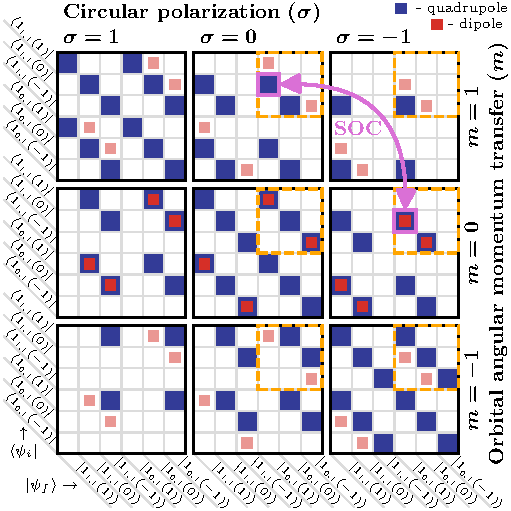
\includegraphics[width=\linewidth]{Figure1.pdf}
    \caption{Allowed dipole (red squares) and quadrupole transitions (blue squares) between eigenstates of the asymmetric top Hamiltonian. Panel columns represent different circular polarizations of the beam, and panel rows -- the amount of the OAM that can be transferred from the beam to the internal rotation of the molecule. Purple circles show an example of spin-orbit coupling creating an \eoet ~term with the transfer of OAM. Orange squares highlight the transitions that would be superimposed in the experiment, as shown in Fig. \ref{fig:profiles}.}
    \label{fig:gridJ1}
\end{figure}

The three columns of Fig.~\ref{fig:gridJ1} correspond to different beam polarizations, and the three rows to different OAM transfer quantum numbers $m$. As shown in Ref.~\cite{Maslov2024,Maslov_Thesis}, electric dipole transitions do not transfer OAM, so they appear only in the $m=0$ row (though we display them in the $m=\pm 1$ rows for comparison). In contrast, electric quadrupole transitions can transfer up to one OAM quantum ($m=0,\pm 1$). Any non-planar beam profile generally contains contributions in all three rows, but their relative weights depend on the specific beam structure.

We first focus on the red-blue squares, indicating pairs of states connected by both dipole and quadrupole transitions. All of these appear in the $m=0$ row, which denotes transitions where no OAM is transferred. This confirms the findings of Table~\ref{SelectionRules} and suggests that for beams with well-defined $\sigma$ the \eoet ~term cannot create HD, but is merely an additional contribution to CD.

However, the clear separation of the OAM in terms of $m$ and the spin in terms of $\sigma$ is only valid for paraxial beams. In fact, any kind of SOC of light would result in a coupling of different $\sigma$ components \cite{Bliokh2015,Bliokh2023}. For our purposes, this means that the terms from different panels in Fig.~\ref{fig:gridJ1} are enabled to drive the same transition. This would, for example, give rise to the \eoet ~term corresponding to the purple square with a transition that is simultaneously dipole (at $m=0$, $\sigma=-1$) and quadrupole (at both $m=0$, $\sigma=-1$ and $m=1$, $\sigma=0$): $| 1_{0,1}(1) \rangle \to | 1_{1,1}(0) \rangle$. The coupling of the dipole moment term to $m=-1$ quadrupole component enables the molecule to sense the impact of OAM.



%%%%%%%%%%%%%%%%%%%%%%%%%%%%%%%%%%%%%%%%%%%%%%%%%%%%
%              DICHROISM CONTRIBUTIONS
%%%%%%%%%%%%%%%%%%%%%%%%%%%%%%%%%%%%%%%%%%%%%%%%%%%%

The spin-orbit coupling of light, required to realize such transitions, can be achieved by tightly--focused Laguerre-Gaussian beams \cite{Loeffler2011,Forbes2021nonparaxial,Forbes2021longitudinal}. Here, we describe the beam in the first--order non-paraxial approximation \cite{Lax1975} (for details see \cite{Note1}), and use the interaction Hamiltonian of Ref.~\cite{Maslov2024,Maslov_Thesis} to calculate the spatially-resolved matrix elements between the states denoted by a dashed square in Fig.~\ref{fig:gridJ1}. The chosen parameters are transition quadrupole moment $Q_{xy}=0.5d_z\lambda$, where $d_z$ is the transition dipole moment and $\lambda$ the wavelength, focal beam-waist $\omega_0=0.2\lambda$, distance from focus $z=\lambda$, with $z$ being the propagation direction, azimuthal charge of the Laguerre-Gausian $L_{\rm beam}=1$ and polarization $\sigma=-1$. The opposite enantiomers are described by reflection on the molecule fixed (inertial) $xy$-plane. It is well-enstablished \cite{Buckingham1971, Power1975} that an anisotropy is needed to observe the \eoet~ interaction, which is why $M$ state resolution is required in any proposed HD experiment. The obtained signal profiles for states with resolved $M$ are shown in Fig.~\ref{fig:profiles}.

\begin{figure}[t!]
    \centering
    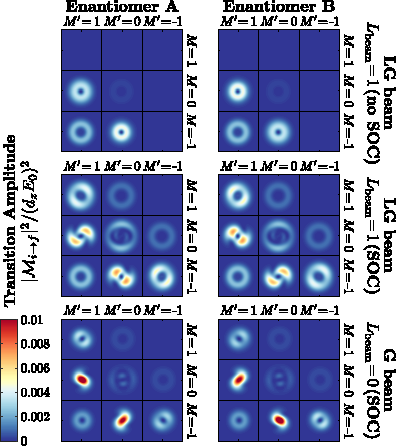
\includegraphics[width=1.0\columnwidth]{Figure2.pdf}
    \caption{Signal profiles of the \eoet ~transitions from $\bra{1_{1,1}(M)}$ to $\ket{1_{0,1}(M')}$ for the opposite enantiomers coupled by a Laguerre Gaussian beam without (top) and with (middle row) the spin-orbit coupling and by a Gaussian beam with spin-orbit coupling (bottom).}
    \label{fig:profiles}
\end{figure}

We first note that the integral of all shown profiles is equal, unless $d_zQ_{xy}^*$ has an imaginary component ${\rm Im}[d_zQ_{xy}^*]$, which leads to dichroism on the level of total absorption. This is a known source of vibrational CD, and is independent of the structure of the electric field and only depends on the internal parameters of the molecule, see \cite{Buckingham1971}. From this result we conclude that HD is impossible to detect by just the magnitude of the absorbed intensity of light, but requires the spatial resolution of the absorption profile~\cite{Loeffler2011}.

Without the light SOC, the only difference between the two enantiomers is the intensity of the $M=0\to M'=1$ and $M=-1\to M'=0$ profiles, see top row of Fig.~\ref{fig:profiles}. This dichroism originates from the $m=0$ part of the beam -- the red-blue squares within the dashed square in the $\sigma=-1$, $m=0$ panel of Fig.~\ref{fig:gridJ1}. Therefore, this is another source of spatially-resolved vibrational CD, as no OAM is transferred. 

The focal field introduces SOC of light, which gives rise to new distinguishing effects between the enantiomers in the absorption profiles, seen in the middle row of Fig.~\ref{fig:profiles}. First, there is a large difference in the absorption of $M=-1\to M'=0$ and $M=0\to M'=1$ transitions. The signal comes from coupling the dipole and quadrupole transitions in the dashed squares in Fig.~\ref{fig:gridJ1}. This difference stems from the relative handedness of the vortex beam and the chiral molecule and involves transfer of OAM. Therefore, this can be considered genuine HD.

Next, there is also a difference in the $M=1\to M'=1$ and $M=-1\to M'=-1$ profiles. This arises from the coupling of dipole transitions in the dashed squares with $\sigma=0$ (Fig.~\ref{fig:gridJ1}) with the quadrupole transitions in the $m=-1$, $\sigma=-1$ square. Therefore, this is also HD. Overall, the dichroism signal in the case of SOC light is an order of magnitude stronger than without the coupling.

The bottom row in Fig. \ref{fig:profiles} shows that in the case of SOC, it is not necessary to use a beam with OAM in the asymptotic limit. Indeed, HD is also observed in the case of a tight focused Gaussian beam. This is because the focal field takes the form of LG mode of azimuthal charge $\sigma$. In fact, a similar dichroism is also seen for a tight focused linearly polarized beam, because the two components of circular polarization within it couple through the SOC. This shows that neither OAM nor spin of the incoming beam are an essential component to observe HD, but rather the SOC.

Note, that due to the SOC of light the type of angular momentum transferred to the molecule cannot be easily distinguished which hinders the characterization of the resulting dichroism as either CD or HD. Our work pinpoints the OAM and spin absorption channels in terms of the quantum numbers $m$ and $\sigma$ (see Fig.~\ref{fig:profiles}) providing a way to resolve this issue.




%%%%%%%%%%%%%%%%%%%%%%%%%%%%%%%%%%%%%%%%%%%%%%%%%%%%
%              CONCLUSION
%%%%%%%%%%%%%%%%%%%%%%%%%%%%%%%%%%%%%%%%%%%%%%%%%%%%

In summary, we have shown that paraxial OAM beams cannot produce HD, as any observed dichroism under these conditions reduces to standard CD. Genuine HD -- dichroism directly tied to the transfer of OAM -- requires spin–orbit coupling of light, as in tightly focused beams. Strikingly, a purely Gaussian mode can exhibit genuine HD once sufficiently focused, even though it carries no OAM in the far-field. These findings clarify the origin of HD in structured-light experiments and suggest that prior measurements of HD may warrant a careful re-examination to confirm the presence of OAM transfer. In particular, the studies that did not observe dichroism were either probing primarily dipole-order interactions \cite{Araoka2005} or lost the dichroism signal due to averaging \cite{Loeffler2011}. The studies that successfully detected dichroism, on the other hand, employed both quadrupole field interactions and tightly focused beams \cite{Rusak2019,Rouxel2022,Begin2023,Jain2023}. 

The framework developed here offers a roadmap for designing chiral-sensitive spectroscopy and enantiomer separation methods leveraging the spatial structure of light~\cite{Leibscher2022}.\\

\begin{acknowledgments}
This research was funded in whole or in part by the Austrian Science Fund (FWF) [10.55776/F1004].  
\end{acknowledgments}



\bibliography{bibliography}




\end{document}